%% Bookheader, Nov 8, 2020; July 18, 2022

\documentclass[11pt]{../Support/ourbook}
%% or for landscape, comment out line above and use this one:
%%\documentclass[landscape,11pt]{ourbook}

%% This will keep space from stretching around display math:

\makeatletter
\renewcommand\normalsize{%
   \@setfontsize\normalsize\@xipt{13.6}%
   \abovedisplayskip 11\p@  \@minus6\p@
   \abovedisplayshortskip \z@ 
   \belowdisplayshortskip 6.5\p@ \@minus3\p@
   \belowdisplayskip \abovedisplayskip
   \let\@listi\@listI}
\makeatother
\normalsize


\begin{document}

\tableofcontents
\graphicspath{{../../Chapters/graphs/en_US}}
\chapter{Introduction to Graphs}

Some data is easiest to work with if we imagine it as a set of \newterm{nodes} connected by \newterm{edges}.  For example,  on some social networks each user can follow any number of other users.  We can think of each user as node and the edge points from the user who follows to the user they follow:

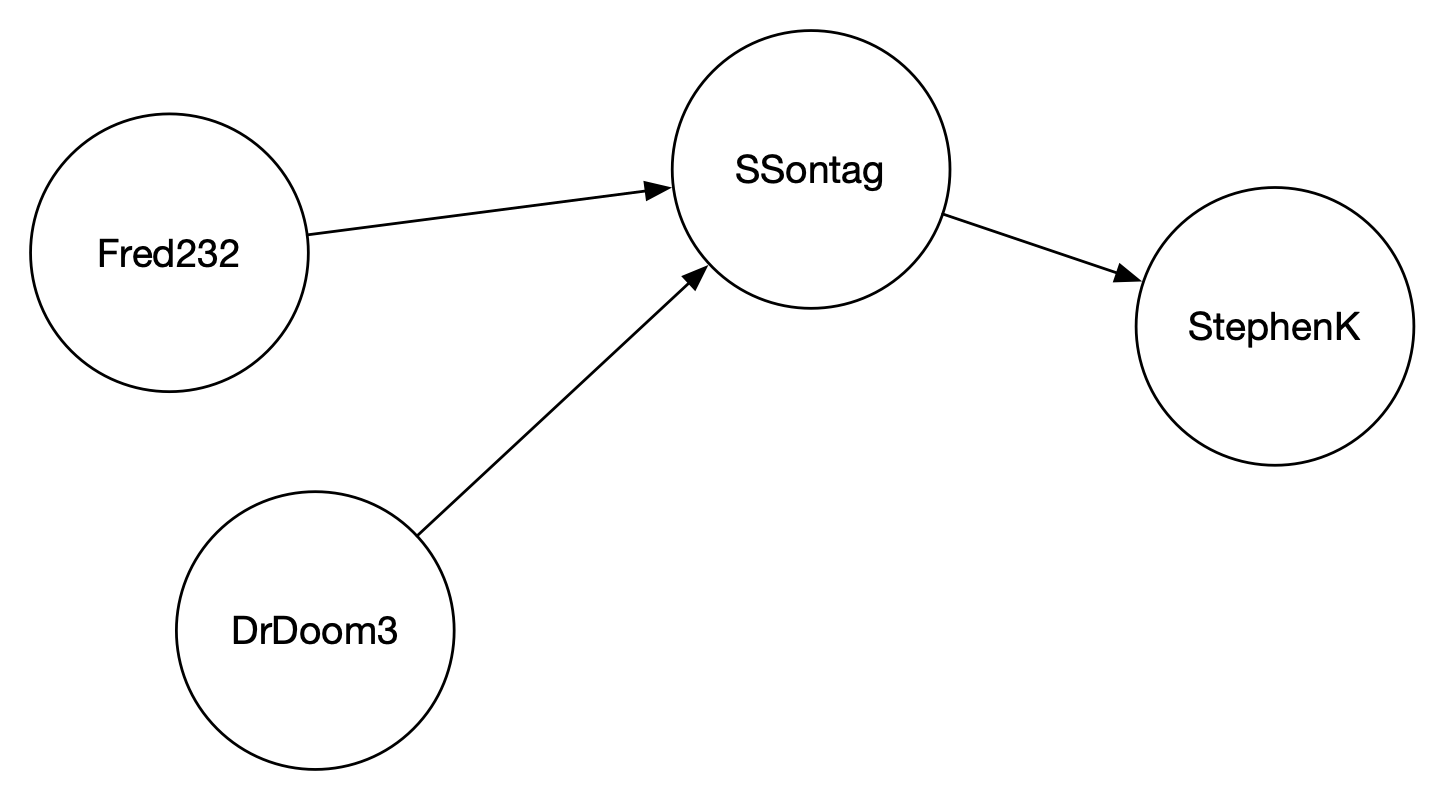
\includegraphics[width=0.7\textwidth]{simpledirected.png}

This diagram shows four users and three follows.   Following  is a directed relationship: Fred232 follows SSontag, but SSontag doesn't follow Fred232.   So we would way that this is a \newterm{directed graph} with four nodes and three edges.

There are also undirected graphs.  for example,  you can imagine a graph that represents big data lines between cities.  All the big data lines allow communications in both directions:

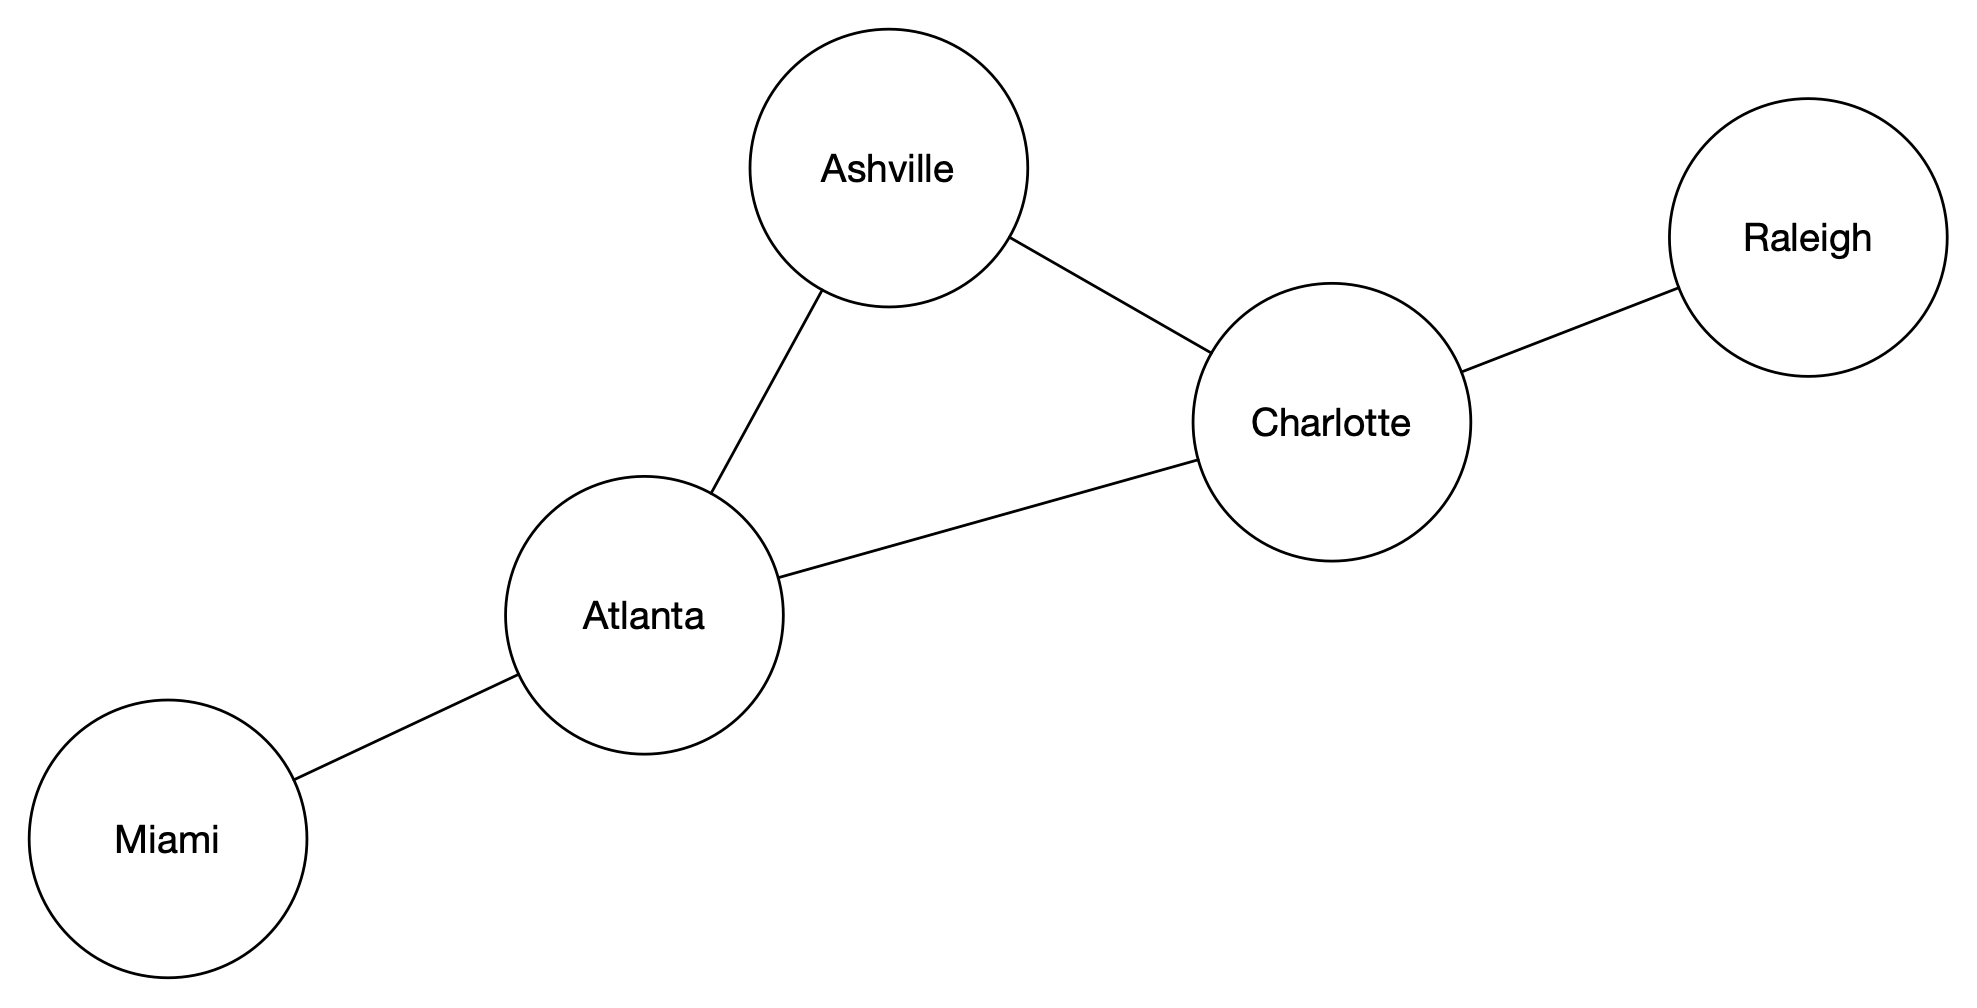
\includegraphics[width=0.7\textwidth]{simpleundirected.png}

The arrows are gone: if data can flow from Charlotte to Raleigh, then data can flow from Raleigh to Charlotte.

There is a whole branch of mathematics called \newterm{Graph Theory} that studies the properties of graphs.  Here are two questions that we might ask about this graph:
\begin{itemize}
\item What is the shortest number of edges that we would need to follow to get from Miami to Raleigh?
\item Does the graph have any paths where you could end up where you started? This is called a \newterm{cycle}.  This graph has one cycle: Atlanta $\rightarrow$ Asheville $\rightarrow$ Charlotte $\rightarrow$ Atlanta.
\end{itemize}

There are even database systems that are specifically designed to hold and analyze graph data.  Not surprisingly,  these are called \newterm{Graph Databases}.

Some graphs are \newterm{connected}: you can get from one node to any other node by following edges.  Is this graph connected?

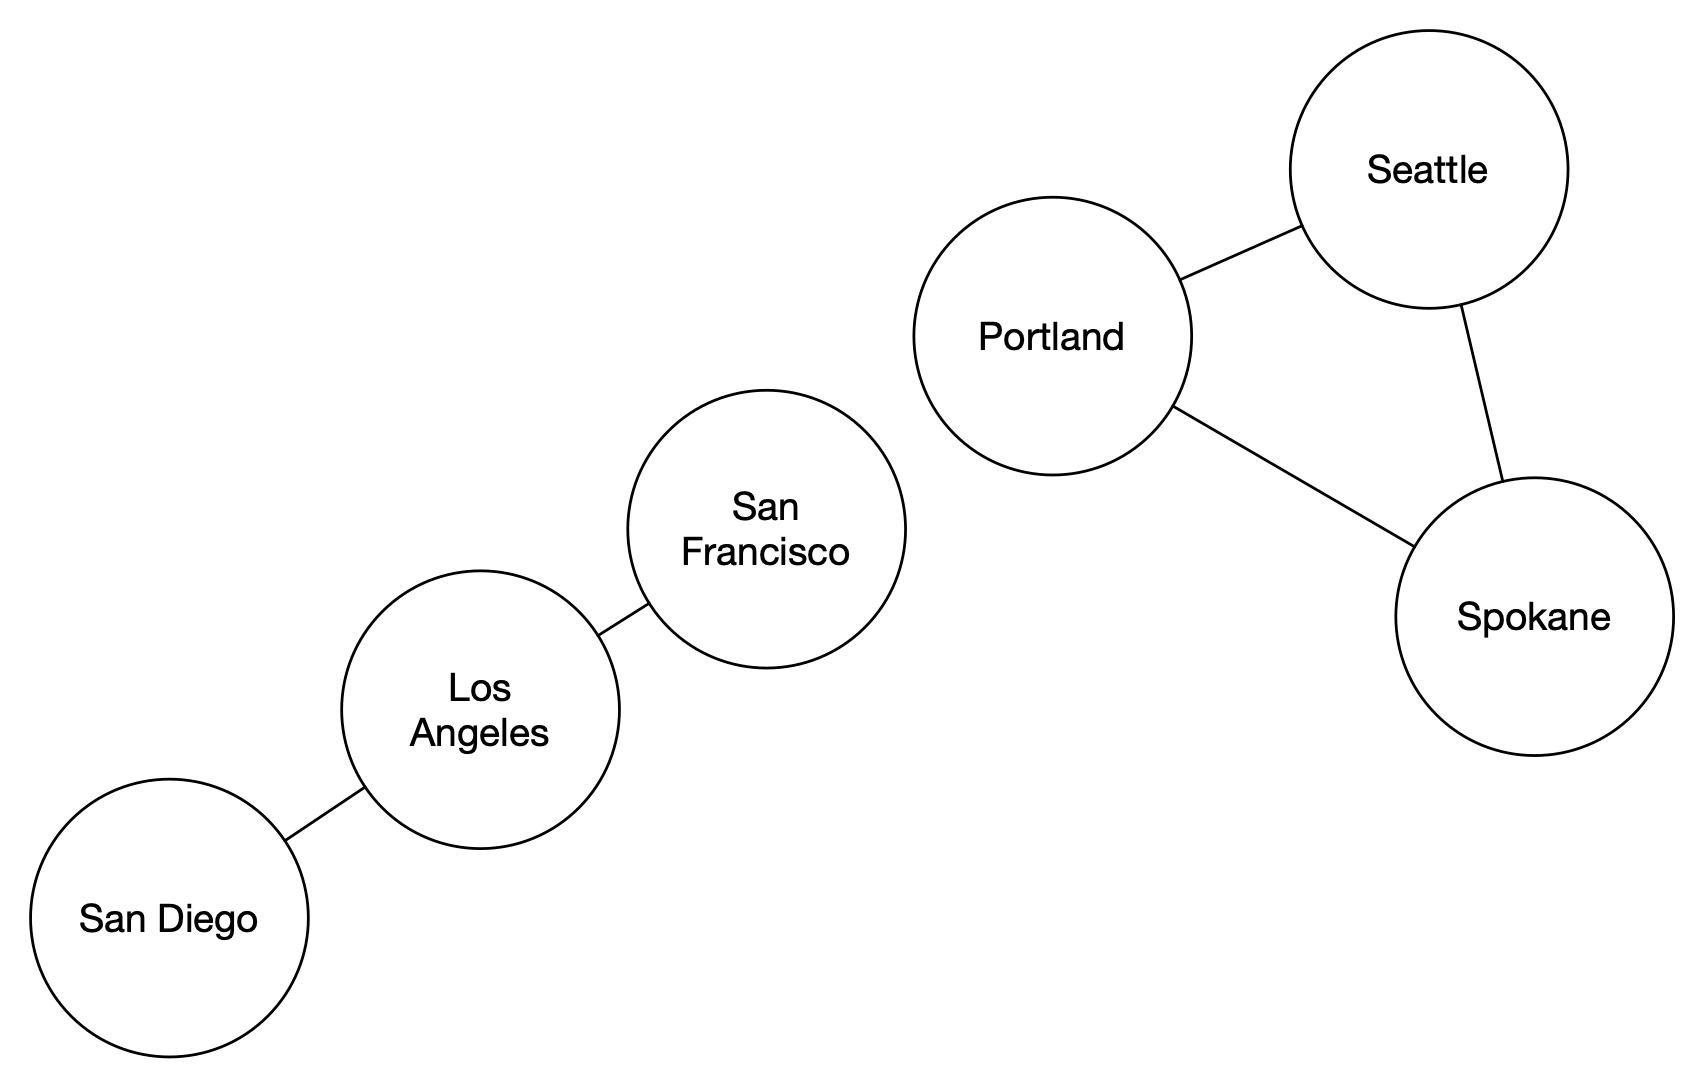
\includegraphics[width=0.7\textwidth]{notconnected.png}

This graph is \textit{not} connected! You can't follow edges from San Diego to Seattle.

In graph data, the nodes and edges often have attributes.  For
example, a node representing a city might have a name and a
population.  An edge representing a data line might have a bandwidth
(bits per second) and a latency (how many nanoseconds between when you
put a bit into the pipe and when it comes out the other end.).

\section{Finding Good Paths}

For a lot of problems, we are trying to find the best path from one
node to another.  If all the edges are the same, this usually means
finding the path that requires walking the fewest edges.

Sometimes the edges have a cost attribute.  For example, you might
want to find the cheapest way to ship a container from New York City
to Long Beach, Calif.  In this case the nodes are train depots.  Each
train line between the depots has a cost.  What is the cheapest path?

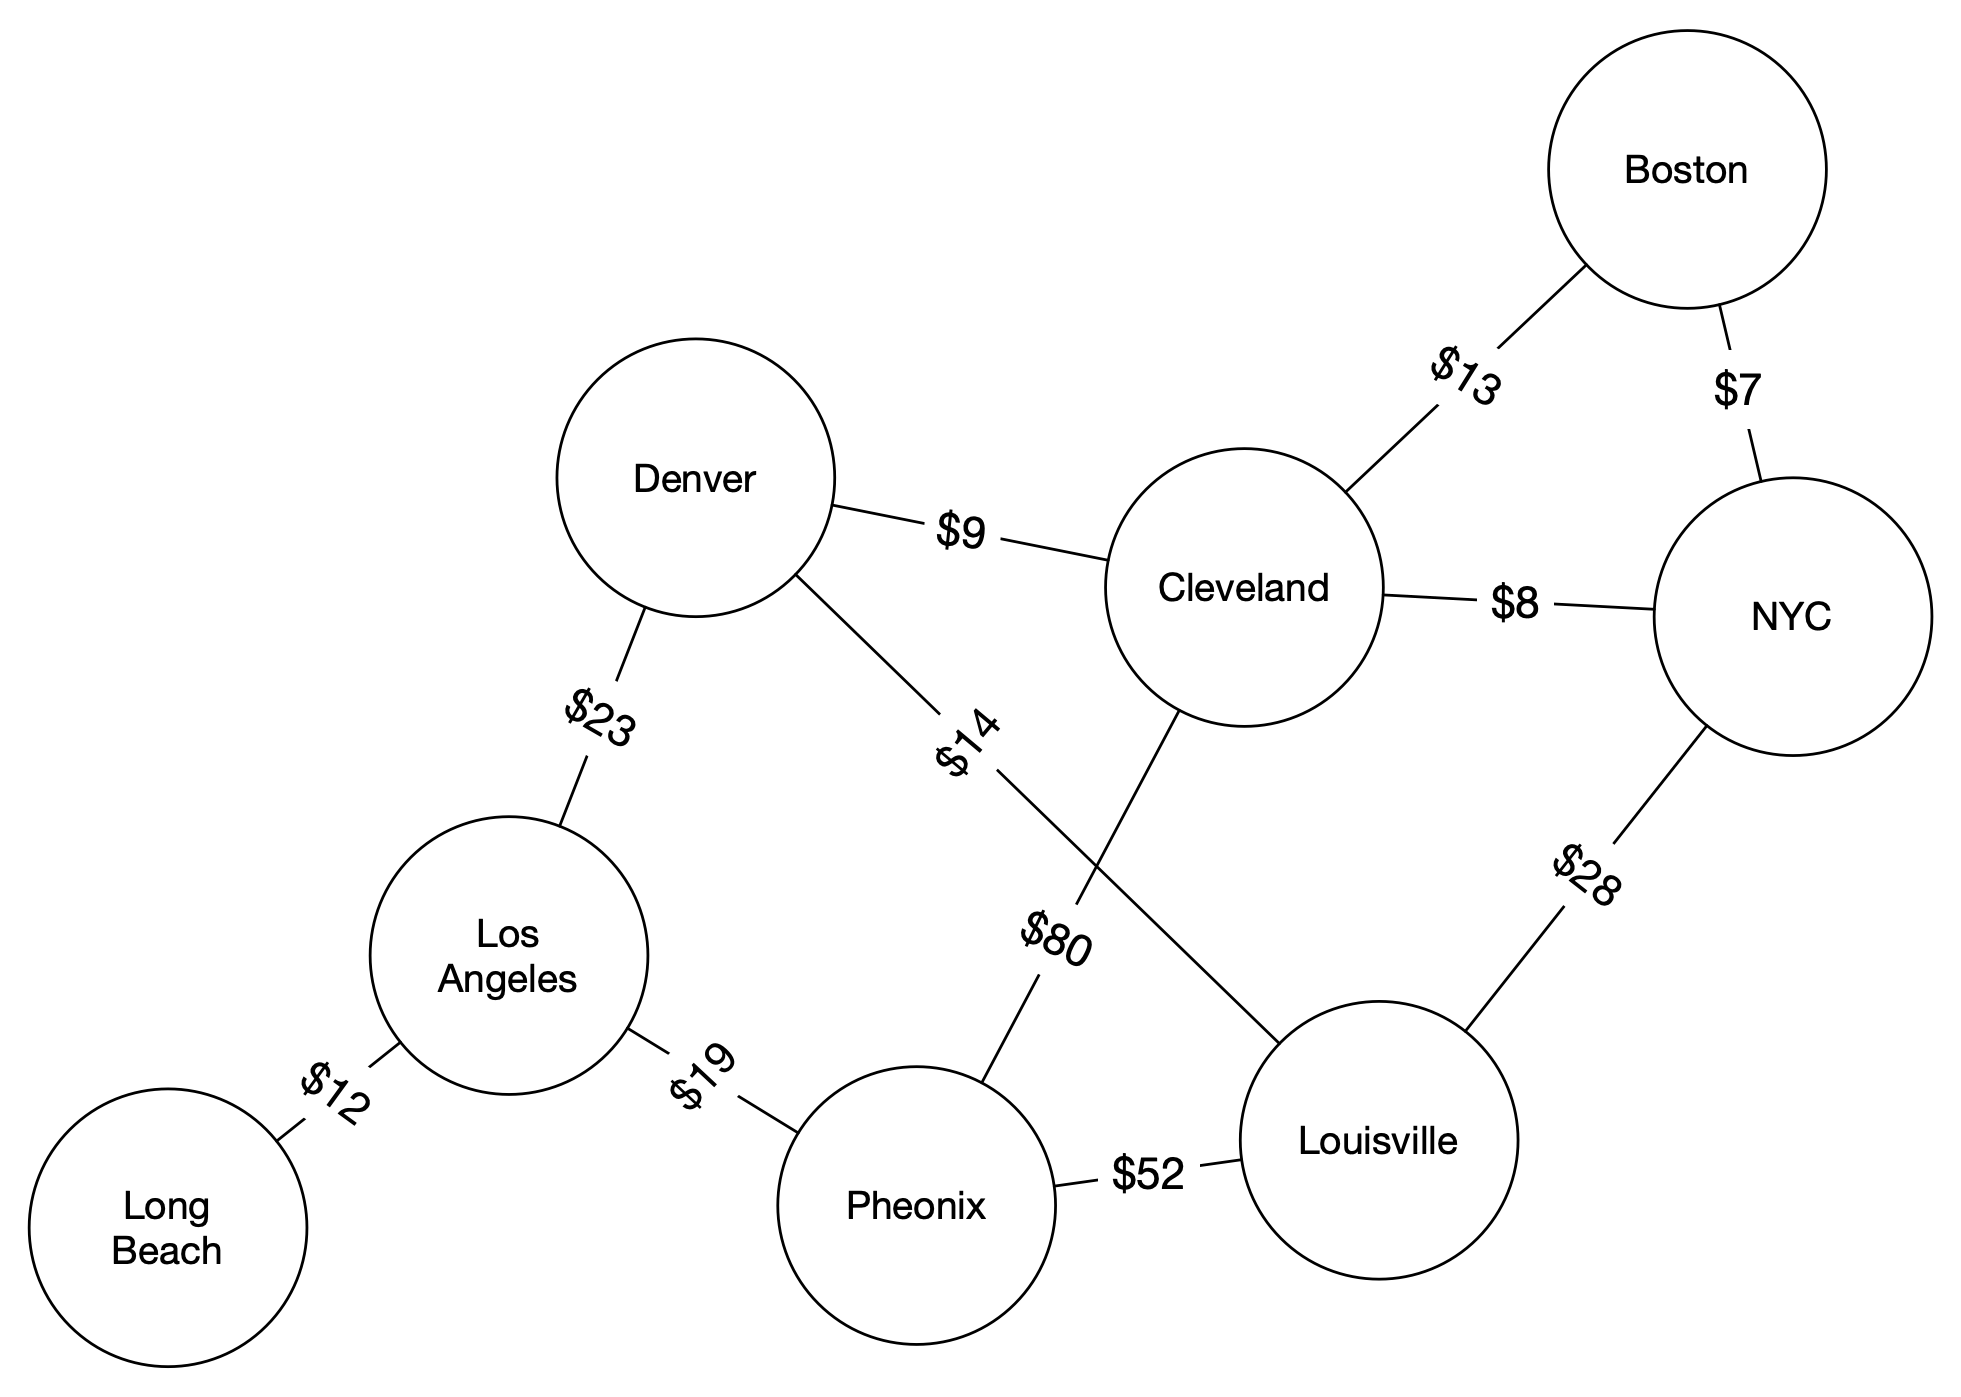
\includegraphics[width=0.7\textwidth]{depots.png}

When edges have costs like this,  we call the \newterm{weighted edges}.

The graphs that you see here are really small, so finding efficient
paths isn't difficult. -- you could just try all of them! However, in
many computer programs, we are working with millions of nodes and
edges.  Efficient graph algorithms are \textit{really} important.

\section{Graphs in Python}

In this section you are going to write Python classes that will let
you represent an undirected graph with weighted edges, like the
shipping problem above.

(Naturally things would look a little different if the graph were
directed or the edges were unweighted, but this is a good starting
place.)

Create a file called \filename{graph.py}.  This will hold the code for
your \pytype{Node} and \pytype{WeightedEdge} classes.  We will also
create a \pytype{Graph} class that will just hold onto the list of
its nodes.

\begin{itemize}
\item A \pytype{Node} will have a label string and a list of edges that touch it.
\item A \pytype{Edge} will have a cost and two nodes: \pyvar{node\_a} and \pyvar{node\_b}.
\item A \pytype{Graph} will have a list of nodes.
\end{itemize}

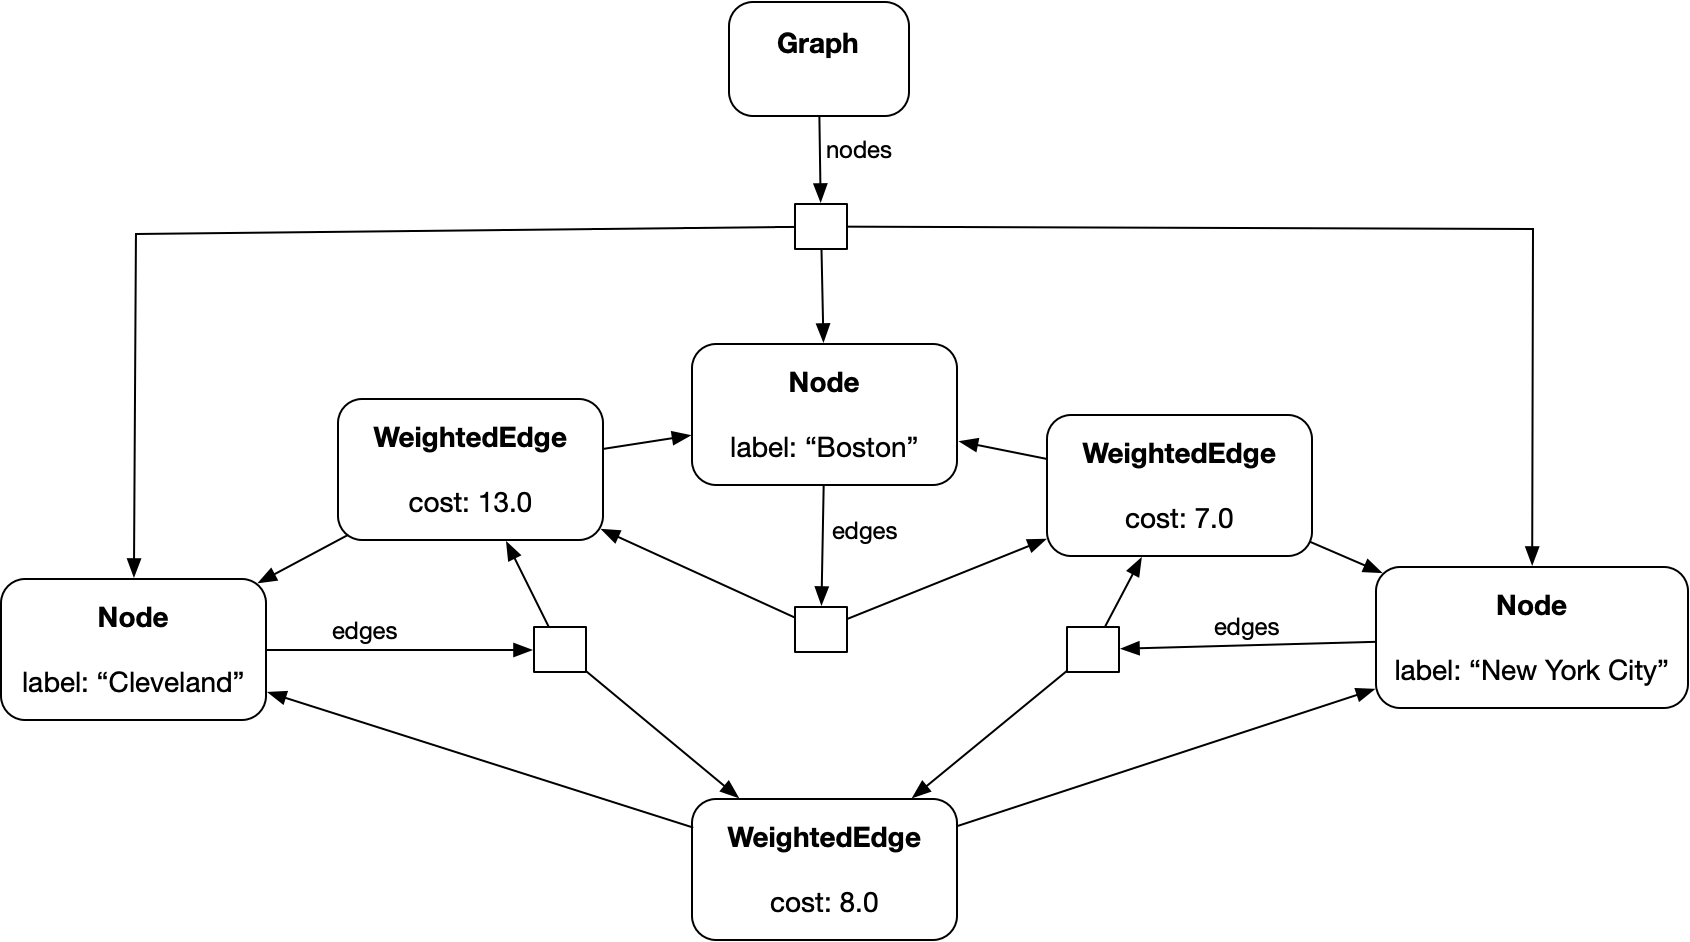
\includegraphics[width=0.8\textwidth]{objdiagram.png}

Put this code into \filename{graph.py}

\begin{verbatim}
class Node:
    def __init__(self, label):
        self.label = label
        self.edges = []

    def __repr__(self):
        return f"(node:{self.label}, edges:{len(self.edges)})"

class WeightedEdge:
    def __init__(self, cost, node_a, node_b):
        self.cost = cost
        self.node_a = node_a
        node_a.edges.append(self)
        self.node_b = node_b
        node_b.edges.append(self)

    def other_end(self, node_from):
        if self.node_a == node_from:
            return self.node_b
        else:
            return self.node_a

class Graph:
    def __init__(self):
        self.nodes = []

    def add_node(self, new_node):
        self.nodes.append(new_node)

    def __repr__(self):
        return f"(Graph:{self.nodes})"
\end{verbatim}

Now lets create some instances of \pytype{Node} and
\pytype{WeightedEdge} and wire them together.  Create another file in
the same directory called \filename{cities.py}. Put in this code:

\begin{verbatim}
import graph

# Create an empty graph
network = graph.Graph()

# Create city nodes and add to graph
long_beach = graph.Node("Long Beach")
network.add_node(long_beach)
los_angeles = graph.Node("Los Angeles")
network.add_node(los_angeles)
denver = graph.Node("Denver")
network.add_node(denver)
pheonix = graph.Node("Pheonix")
network.add_node(pheonix)
louisville = graph.Node("Louisville")
network.add_node(louisville)
cleveland = graph.Node("Cleveland")
network.add_node(cleveland)
boston = graph.Node("Boston")
network.add_node(boston)
nyc = graph.Node("New York City")
network.add_node(nyc)

# Create edges
graph.WeightedEdge(12, long_beach, los_angeles)
graph.WeightedEdge(23.0, los_angeles, denver)
graph.WeightedEdge(19, los_angeles, pheonix)
graph.WeightedEdge(52, pheonix, louisville)
graph.WeightedEdge(14, denver, louisville)
graph.WeightedEdge(80, pheonix, cleveland)
graph.WeightedEdge(9, denver, cleveland)
graph.WeightedEdge(8, cleveland, nyc)
graph.WeightedEdge(28, louisville, nyc)
graph.WeightedEdge(7, nyc, boston)
graph.WeightedEdge(13, cleveland, boston)

print(network)
\end{verbatim}

Run it:
\begin{verbatim}
python3 cities.py
\end{verbatim}

You should see some rather unexciting output:

\begin{verbatim}
(Graph:[(node:Long Beach, edges:1), (node:Los Angeles, edges:3), (node:Denver, edges:3),
(node:Pheonix, edges:3), (node:Louisville, edges:3), (node:Cleveland, edges:4),
(node:Boston, edges:2), (node:New York City, edges:3)])
\end{verbatim}

But we will make it more exciting in the next chapter!

\graphicspath{{../../Chapters/dijkstra/en_US}}
\chapter{Dijkstra's Algorithm}

Add a method to the \pytype{Graph} class that implements Dijkstra's algorithm:
\begin{verbatim}
    def cost_from_node(self, origin_node):
        # Cost of cheapest path from origin node discovered so far
        dist = {k: math.inf for k in self.nodes}

        # The previous city on that cheapest path
        prev = {}

        # All the nodes start as unvisited
        unvisited = set(self.nodes)
    
        # The distance from the origin node to itself is zero
        dist[origin_node] = 0.0

        # While there are still unvisited nodes
        while unvisited:

            # Find unvisited node with lowest cost
            min_cost = math.inf
            for u in unvisited:
                if dist[u] < min_cost:
                    current_node = u
                    min_cost = dist[u]

            # If none are less than inf, we are done
            # This happens in graphs that are not connected
            if min_cost == math.inf:
                return (dist, prev)
            
            # Remove the lowest cost node from the unvisited list
            unvisited.remove(current_node)

            # Update all the unvisited neighbors
            for edge in current_node.edges:

                # What node is at the other end of this edge?
                v = edge.other_end(current_node)

                # Visited nodes are already minimized, skip them
                if v not in unvisited:
                    continue

                # Is this a shorter route?
                alt = dist[current_node] + edge.cost
                if alt < dist[v]:

                    # Update the distance and prev dicts
                    dist[v] = alt
                    prev[v] = current_node

        return (dist, prev)
\end{verbatim}

Append some code to your \filename{cities.py} that test this method:

\begin{verbatim}
(cost_from_long_beach, prev) = network.cost_from_node(long_beach)
print(f"\nMinimum costs from Long Beach = {cost_from_long_beach}")
print(f"\nLast city before = {prev}")

nyc_cost = cost_from_long_beach[nyc]

if nyc_cost < math.inf:
    print(f"\n*** Total cost from Long Beach to NYC: ${nyc_cost:.2f} ***")
else:
    print("You can't get to NYC from Long Beach")
\end{verbatim}

When you run it, you should get a list of how much it costs to ship a
container to each city from Long Beach:
\begin{verbatim}
Minimum costs from Long Beach = {(node:Long Beach, edges:1): 0.0,
(node:Los Angeles, edges:3): 12.0, (node:Denver, edges:3): 35.0,
(node:Pheonix, edges:3): 31.0, (node:Louisville, edges:3): 49.0,
(node:Cleveland, edges:4): 44.0, (node:Boston, edges:2): 57.0,
(node:New York City, edges:3): 52.0}
\end{verbatim}

You will also get a collection of node pairs. What are these? For each
node, you get the node that you would pass through on the cheapest
route from Long Beach:
\begin{verbatim}
Last city before = {(node:Los Angeles, edges:3):(node:Long Beach, edges:1),
(node:Denver, edges:3):(node:Los Angeles, edges:3),
(node:Pheonix, edges:3):(node:Los Angeles, edges:3),
(node:Louisville, edges:3):(node:Denver, edges:3),
(node:Cleveland, edges:4):(node:Denver, edges:3),
(node:New York City, edges:3):(node:Cleveland, edges:4),
(node:Boston, edges:2): (node:Cleveland, edges:4)}
\end{verbatim}

Your users won't want to read this; Give them the shortest path as a list.  Add a function to
\filename{graph.py} that turns the \pyvar{prev} table into a path of
nodes that lead from the origin to the destination:

\begin{verbatim}
def shortest_path(prev, destination):

    # Include the destination in the path
    path = [destination]
    current_node = destination

    # Keep stepping backward in the path
    while current_node in prev:

        # What node should come before the current node?
        previous_node = prev[current_node]

        # Insert it at the start of the list
        path.insert(0, previous_node)
        current_node = previous_node

    return path
\end{verbatim}

Test that out:

\begin{Verbatim}[commandchars=\\\{\}]
if nyc_cost < math.inf:
    print(f"*** Total cost from Long Beach to NYC: ${nyc_cost:.2f} ***")

    \textbf{path_to_nyc = graph.shortest_path(prev, nyc)}
    \textbf{print(f"*** Cheapest path from Long Beach to NYC: {path_to_nyc} ***")}
else:
    print("You can't get to NYC from Long Beach")
\end{Verbatim}

This should look like this:
\begin{verbatim}
*** Cheapest path from Long Beach to NYC: [(node:Long Beach, edges:1),
(node:Los Angeles, edges:3), (node:Denver, edges:3), (node:Cleveland, edges:4),
(node:New York City, edges:3)] ***
\end{verbatim}

\graphicspath{{../../Chapters/binary_search/en_US}}
\chapter{Binary Search}

As mentioned in the last chapter, you are going to make a priority
queue for use with Dijkstra's Algorithm.  Using it will look like this:

\begin{verbatim}
import kpqueue

myqueue = pqueue.PriorityQueue()
myqueue.add(long_beach, 0) # Inserts first city and its cost
myqueue.add(san_diego, 14) # Puts San Diego after Long Beach
myqueue.add(los_angeles,12) # Inserts LA between Long Beach and San Diego
current_city = myqueue.pop() # Returns first city (Long Beach) and removes it
\end{verbatim}

Now if an item gets a new priority, we need to remove it and reinsert it in the new spot.
\begin{verbatim}
myqueue.add(city_a, 16) # Puts it last in the queue
myqueue.update(city_a, 16, 13) # Moves it to between LA and San Diego
\end{verbatim}

\section{A Naive Implementation of the Priority Queue}

Create a file called \filename{kpqueue.py}. Let's do a simple
implementation that stores the priority and the data as tuple. And we
will keep it sorted by the priority.  If two tuples have the same
priority, we'll sort by the data.

Type this in to \filename{kpqueue.py}:
\begin{verbatim}
class PriorityQueue:
    def __init__(self):
        self.list = []
    
    # Return and remove the first item
    def pop(self):
        if len(self.list) > 0:
            return self.list.pop(0)
        else:
            return None
        
    def __len__(self):
        return len(self.list)

    def update(self, value, old_priority, new_priority):
        old_pair = (old_priority, value)
        self.list.remove(old_pair)
        self.add(value, new_priority)
    
    def add(self, value, priority):
        pair = (priority, value)
        # Add it at the end
        self.list.append(pair)
        # Resort the list
        self.list.sort()
\end{verbatim}

This will work fine, but it could be much more efficient:
\begin{itemize}
\item Every time we add a single element, we resort the whole list.
\item The function \pyfunction{remove} is searching the list sequentially for the item to delete.
\end{itemize}

In a minute, we will revisit these inefficiencies and make the better.

\section{Using the Priority Queue}

We are going to change \filename{graph.py} to use the priority
queue. While we are doing, why don't we also shrink the memory
footprint of our program a bit.

Notice that as the algorithm is running, each node is in one of three states:
\begin{itemize}
\item Unseen: In the earlier implementation, these were the nodes with \pyvar{math.inf} as their cost.
\item Seen, but not finalized: These are ``unvisited'' but don't have \pyvar{math.inf} as their cost.
\item Finalized: These are the ``visited'' nodes -- we know that their cost won't decrease any more.
\end{itemize}

We can shrink the memory foot print by not putting the unseen into the
dist dictionary at all. And instead of a separate set for
``unvisited'' what if we moved finalized nodes and their distances
into a separate dictionary?

Rewrite the \pyfunction{cost\_from\_node} function in \filename{graph.py}:

\begin{verbatim}
              # Visited nodes are already minimized, skip them
                if v in finalized_dist:
                    continue

                # What is the cost to this neighbor?
                alt = current_node_cost + edge.cost

                # Is this the first time I am seeing the node?
                if v not in seen_dist:

                    # Insert into the seen_dict, prev, and priority queue
                    seen_dist[v] = alt
                    prev[v] = current_node
                    pqueue.add(v, alt)

                else: # v has been seen. Is this a cheaper route?
                    old_dist = seen_dist[v]
                    if alt < old_dist:
                        # Update the seen_dict, prev, and priority queue
                        seen_dist[v] = alt
                        prev[v] = current_node
                        pqueue.update(v, old_dist, alt)

        return (finalized_dist, prev)
\end{verbatim}

This should be have exactly the same except for the unreachable nodes.
If you have a graph that is not connected, there will be nodes that
can't be reached from the origin.  In the old version, these had a
cost of \pyvar{math.inf}.  Now they just won't be in the dictionary at all.  So, change \filename{cities.py} to deal with this:

\begin{verbatim}
if nyc in cost_from_long_beach:
    nyc_cost = cost_from_long_beach[nyc]
    print(f"\n*** Total cost from Long Beach to NYC: ${nyc_cost:.2f} ***")

    path_to_nyc = graph.shortest_path(prev, nyc)
    print(f"\n*** Cheapest path from Long Beach to NYC: {path_to_nyc} ***")
else:
    print("You can't get to NYC from Long Beach")
\end{verbatim}

If you run \filename{cities.py} now, it should behave exactly like the old version.

But there is a bug. It will rear its head if two cities with the same
cost are in the priority queue together.  Change \filename{cities.py}
so that Denver and Pheonix have the same cost:

\begin{verbatim}
graph.WeightedEdge(12, long_beach, los_angeles)
graph.WeightedEdge(19, los_angeles, denver)
graph.WeightedEdge(19, los_angeles, pheonix)
\end{verbatim}

Now try running it.  You should get an error:

\begin{verbatim}
TypeError: '<' not supported between instances of 'Node' and 'Node'
\end{verbatim}

What happened? The \pyfunction{loc\_for\_pair} method is comparing
tuples made up of a \pytype{float} and a \pytype{Node}.  The
\pytype{float} comes first in the tuple, so that is compared
first. However, if the two tuples have the same priority, it then
compares nodes.

The error statement say ``Nodes don't have a less-than method; I don't
know how to compare them.''

Each \pytype{Node} lives at an address in memory. You can get that
address as a number using the \pyfunction{id} function. The ID is
unique and constant over the life of the object. It is a rather
arbitary ordering, but it will work for this problem.  Add a method to
your \pytype{Node} class:

\begin{verbatim}
    # Nodes will be ordered by their location in memory
    def __lt__(self, other):
        return id(self) < id(other)
\end{verbatim}

Fixed.

Now let's make the priority queue more efficient.

\section{Binary Search}

The phone company in every town used to print a thing called a phone
book. The names and phone numbers were arranged alphabetically.  As
you might imagine, these books often had more than a thousand pages.

If you were looking for ``John Jeffers'', you wouldn't start at the
first page and read sequentially until you reached his name.  You
would open the book in the middle, and see a name like ``Mac Miller'',
and then think ``Jeffers comes before Miller''.  Then you would split
the pages in your left hand in half and see a name like ``Hester
Hamburg'' and think ``Jeffers comes after Hamburg''.  Then you would
split the pages in your right hand, and so on until you found the page
with ``John Jeffers'' on it.

That is binary search.

Binary Search is a search algorithm that finds the position of a target value within a sorted array. The binary search algorithm works by repeatedly dividing the search interval in half. If the target value is equal to the middle element of the array, the position is returned. If the target value is less or greater than the middle element, the search continues in the lower or upper half of the array respectively.

\section{Algorithm}

The binary search algorithm can be described as follows:

\begin{enumerate}
\item If the array is empty, the search is unsuccessful, so return "Not Found".
\item Otherwise, compare the target value to the middle element of the array.
\item If the target value matches the middle element, return the middle index.
\item If the target value is less than the middle element, repeat the search with the lower half of the array.
\item If the target value is greater than the middle element, repeat the search with the upper half of the array.
\item Repeat steps 2-5 until the target value is found or the array is exhausted.
\end{enumerate}


\begin{verbatim}
class PriorityQueue:
    def __init__(self):
        self.list = []
    
    # Return and remove the first item
    def pop(self):
        if len(self.list) > 0:
            return self.list.pop(0)
        else:
            return None
        
    def __len__(self):
        return len(self.list)
    
    def add(self, value, priority):
        pair = (priority, value)
        i = self.loc_for_pair(pair)
        self.list.insert(i, pair)

    def update(self, value, old_priority, new_priority):
        old_pair = (old_priority, value)
        i = self.loc_for_pair(old_pair)
        del self.list[i]
        self.add(value, new_priority)
    
    def loc_for_pair(self, pair):
        # The range where it could be is [lower, upper)
        # Start with the whole list
        lower = 0
        upper = len(self.list)

        while upper > lower:
            next_split = (upper + lower) // 2
            v = self.list[next_split]    
            if pair < v:  # pair is to the left
                upper = next_split
            elif pair > v:  # pair is to the right
                lower = next_split + 1
            else: # Found pair!
                return next_split
        return lower
\end{verbatim}

If you try running it now, it should work perfectly.

Now you have a graph class that would find the cheapest path quickly
even if it had thousands of nodes with thousands of edges.

\graphicspath{{../../Chapters/graph_algorithms/en_US}}
\chapter{Other Graph Algorithms}

Now that you are familiar with Dijkstra's algorithm for finding the
shortest path in a graph, you are well-equipped to understand more
graph algorithms. This document will discuss two other important
algorithms: Depth-First Search (DFS) and the Bellman-Ford algorithm.\index{depth-first search} \index{DFS}

\section{Depth-First Search}

Depth-First Search (DFS) is an algorithm for traversing or searching
tree or graph data structures. DFS uses a stack (or sometimes
recursion, which uses the system stack implicitly) to explore the graph
in a depthward motion until it hits a node with no unvisited adjacent
nodes, then it backtracks.

The procedure is as follows:

\begin{enumerate}
    \item Push the root node into the stack.
    \item Pop a node from the stack, and mark it as visited.
    \item Push all unvisited adjacent nodes into the stack.
    \item Repeat steps 2 and 3 until the stack is empty.
\end{enumerate}

DFS is particularly useful for solving problems like
connected-component detection in graphs and maze-solving.

\section{Bellman-Ford Algorithm}

The Bellman-Ford algorithm is another shortest path algorithm like
Dijkstra's. However, unlike Dijkstra's algorithm, Bellman-Ford can
handle graphs with negative weight edges.\index{Bellman-Ford algorithm}

The algorithm works as follows:

\begin{enumerate}
    \item Assign a tentative distance value for every node: set it to
      zero for our initial node and to infinity for all other nodes.
    \item For each edge $(u, v)$ with weight $w$, if the current
      distance to $v$ is greater than the distance to $u$ plus $w$,
      update the distance to $v$ to be the distance to $u$ plus $w$.
    \item Repeat the previous step $|V| - 1$ times, where $|V|$ is the
      number of vertices in the graph.
    \item After the above steps, if you can still find a shorter path,
      there exists a negative cycle.
\end{enumerate}

If the graph does not contain a negative cycle reachable from the
source, the shortest paths are well-defined, and Bellman-Ford will
correctly calculate them. If a negative cycle is reachable, no
solution exists, but Bellman-Ford will detect it.

\graphicspath{{../../Chapters/bayesian_networks/en_US}}
\chapter{Bayesian Networks}

A Bayesian network, also known as a Bayes network, belief network, or
decision network, is a probabilistic graphical model that represents a
set of variables and their conditional dependencies via a directed
acyclic graph (DAG).\index{Bayesian Network}

\section{Components}

A Bayesian Network consists of two main components:

\begin{enumerate}
    \item A directed acyclic graph (DAG) where each node represents a
      variable, and the absence or presence of a directed edge between
      nodes denotes the conditional dependence or independence
      respectively between the variables.
    \item A conditional probability table (CPT) associated with each
      node which contains the conditional probability distribution of
      that node given its parents in the DAG.
\end{enumerate}

\section{Inferences}

Bayesian Networks are typically used for reasoning and making
inferences under uncertainty. Given observations of a set of
variables, we can compute the posterior probabilities of the other
variables using Bayes' rule.

There are three main types of inferences that we can make:

\begin{itemize}
    \item \textbf{Causal reasoning (prediction)}: Given the causes,
      what are the effects?
    \item \textbf{Evidential reasoning (diagnosis)}: Given the
      effects, what are the causes?
    \item \textbf{Intercausal reasoning (explaining away)}: Given an
      effect and some of its causes, what can we say about the other
      causes?
\end{itemize}

\section{Learning}

Learning a Bayesian Network from data involves two main tasks:

\begin{itemize}
    \item \textbf{Structure learning}: Determining the DAG structure
      that best fits the data.
    \item \textbf{Parameter learning}: Estimating the parameters
      (conditional probabilities) of the CPTs given the DAG and data.
\end{itemize}

%%%%%%%%%%%%%%%%%%%%%%%%%%%%%%%%%
%% Bookfooter.tex by Aaron Hillegass
%% Nov 8, 2020

\appendix

\chapter{Answers to Exercises}
\shipoutAnswer

\bibliography{references}

\printindex

\end{document}